\subsection{Obbiettivi del prodotto}
L'obbiettivo del \glossario{chatbot} è quello di aiutare i dipendenti dell'azienda. Essi potranno fornire dei comandi testuali o vocali in input al  \glossario{chatbot}, guidandoli e semplificando l'esecuzione di alcuni compiti, come: aprire il cancello, tracciare la presenza, 
consuntivare le ore di lavoro, ricercare documenti, programmare una riunione, segnalare e 
tracciare i bug. \newline
Il \glossario{chatbot} potrà essere utilizzato solo dai dipendenti dell'azienda \textit{Imola Informatica}, cioè utenti che dispongono una
mail con dominio \textbf{@imolainformatica.it}

\subsection{Struttura}
Il prodotto avrà come componenti principali:
\begin{itemize}
    \item \textbf{Interfaccia autenticazione:} l'autenticazione avverrà mediante un server esterno che 
                genererà un \glossario{token} di accesso
    \item \textbf{Interfaccia chatbot:} interfaccia messaggistica dell'applicazione in cui l'utente dialoga 
                con il bot tramite input testuale o vocale, resterà traccia del flusso dei messaggi.
    \item \textbf{Web server:} l'intermediario tra le richieste dell'utente e i servizi aziendali, interpreta 
                i messaggi scritti dall'utente e se possibile esegue subito l'azione richiesta altrimenti 
                richiede all'utente altre informazioni più specifiche.
\end{itemize}

\subsection{Vincoli}
Per poter utilizzare il \glossario{chatbot} è necessario un dispositivo (smartphone, tablet o computer) che 
abbia tastiera o microfono e una connessione internet attiva.

\subsection{Attori}
A seguito dell'analisi del capitolato e dagli incontri con Imola Informatica, nel sistema sono 
presenti solo attori primari:
\begin{itemize}
    \item \textbf{Utente non autorizzato:} utente che non è ancora stato identificato come dipendente aziendale e quindi non ha accesso ai servizi offerti dal \glossario{chatbot}, ma solamente al sistema di autenticazione.
    \item \textbf{Utente autorizzato:} l'utente è stato riconosciuto come dipendente aziendale, quindi 
                ha accesso a tutte le funzionalità del \glossario{chatbot}. \newline
                L'utente autorizzato nel \glossario{chatbot} è una generalizzazione di:
                \begin{itemize}
                \item \textbf{utente autorizzato e ha eseguito l'accesso alla piattaforma di riunione}
                \item \textbf{utente autorizzato e non ha eseguito l'accesso alla piattaforma di riunione}
                \end{itemize}
                cioè se è stato effettuato il login anche nella piattaforma (Zoom, Meet, Teams) in 
                cui si programma la riunione.
\end{itemize}

\begin{figure}[h]
    \centering
    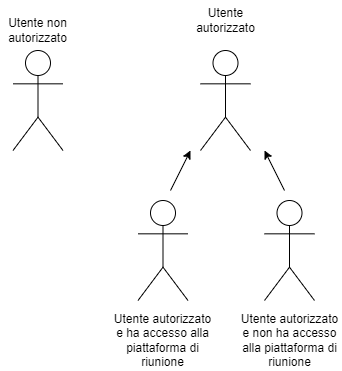
\includegraphics[scale=1]{images/Attori.png} 
    \caption{Rappresentazione grafica degli attori coinvolti all'interno dei casi d'uso}
\end{figure}
\newpage